%%%%%%%%%%%%%%%%%%%%%%%%%%%%%%%%%%%%%%%%%%%%%%%%%%%%%%%%%%%%%%%%%%%%%%
%%                     Association
%%%%%%%%%%%%%%%%%%%%%%%%%%%%%%%%%%%%%%%%%%%%%%%%%%%%%%%%%%%%%%%%%%%%%%

\subsection{Glyph: \glyph{Association}}\label{sec:association}

The association between one or more \glyph{EPNs} represents the non-covalent binding of the biological objects represented by those \glyph{EPNs} into a larger complex. An \glyph{association} between several entities is represented by a filled disc linked to two connectors separated by 180 degrees. The consumption (\sect{consumption}) and production (\sect{production}) arcs are linked to the extremities of those connectors. An \glyph{association} is never reversible, the inverse process being represented by a \glyph{dissociation} (\sect{dissociation}).

\begin{figure}[H]
  \centering
  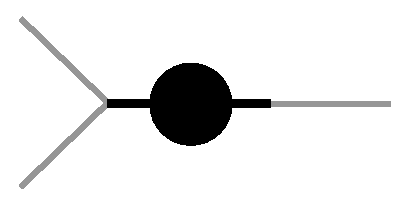
\includegraphics[scale = 0.5]{images/association}
  \caption{The \PD glyph for \glyph{association}.}
  \label{fig:association}
\end{figure}
